\section{Test Result}

\subsection{Overview}
We use the OpenCV library to perform these tests. All the codes are written in C++.
We trained five different models based on five training sets then used five test sets tested them. The tests have great result, which are showed in figure \ref{fig:res:1}

\begin{figure}[H]
\centering
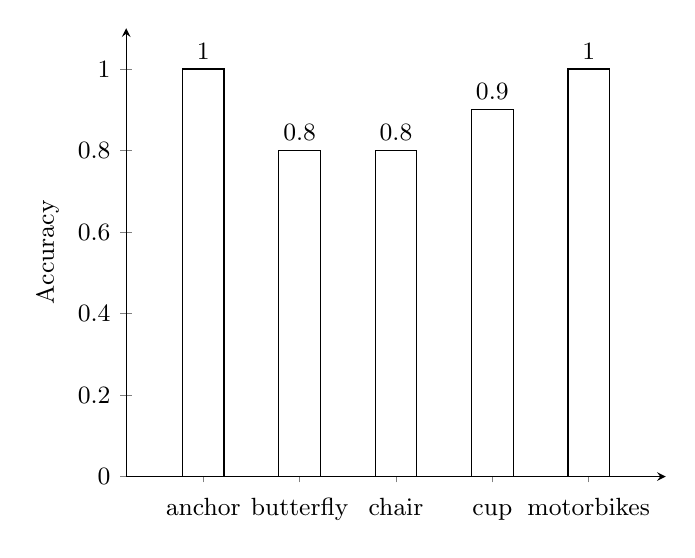
\begin{tikzpicture}[font=\small]
\begin{axis}[
    ybar,
    bar width=15pt,
    ylabel={Accuracy},
    ymin=0,
    ymax =1.1,
    xtick=data,
    axis x line=bottom,
    axis y line=left,
    enlarge x limits=0.2,
    symbolic x coords={anchor,butterfly,chair,cup,motorbikes},
    xticklabel style={anchor=base,yshift=-\baselineskip},
    nodes near coords={\pgfmathprintnumber\pgfplotspointmeta}
]
    \addplot[fill=white] coordinates {
    (anchor,        1.0)
    (butterfly,     0.8)
    (chair,         0.8)
    (cup,           0.9)
    (motorbikes,    1.0)
    };
\end{axis}
\end{tikzpicture}
\caption{Test Result}
\label{fig:res:1}
\end{figure}

%----------------------------------------------------------------------------------------
%	Anchor
%----------------------------------------------------------------------------------------

\subsection{Anchor}

\begin{table}[H]
\centering

\begin{tabular}{|l|l|}
\hline
\textbf{name}                 & \textbf{value} \\ \hline
number of class in clustering & 40             \\ \hline
kernel type                   & RBF            \\ \hline
$\gamma$ of kernel function   & 5              \\ \hline
maximum iterations            & 100            \\ \hline
terminate threshold           & 1e-6           \\ \hline
\end{tabular}
\caption{Parameters of the anchor model.}
\end{table}

The parameter of this model is listed as above.
This model gives a \textbf{1.0} accuracy to the test images of anchors.


%----------------------------------------------------------------------------------------
%	Butterfly
%----------------------------------------------------------------------------------------

\subsection{Butterfly}

\begin{table}[H]
\centering

\begin{tabular}{|l|l|}
\hline
\textbf{name}                 & \textbf{value} \\ \hline
number of class in clustering & 80             \\ \hline
kernel type                   & RBF            \\ \hline
$\gamma$ of kernel function   & 5              \\ \hline
maximum iterations            & 100            \\ \hline
terminate threshold           & 1e-6           \\ \hline
\end{tabular}
\caption{Parameters of the butterfly model.}
\end{table}

The parameter of this model is listed as above.
This model gives a \textbf{0.8} accuracy to the test images of butterflies.


%----------------------------------------------------------------------------------------
%	Chair
%----------------------------------------------------------------------------------------

\subsection{Chair}

\begin{table}[H]
\centering

\begin{tabular}{|l|l|}
\hline
\textbf{name}                 & \textbf{value} \\ \hline
number of class in clustering & 40             \\ \hline
kernel type                   & RBF            \\ \hline
$\gamma$ of kernel function   & 1              \\ \hline
maximum iterations            & 100            \\ \hline
terminate threshold           & 1e-6           \\ \hline
\end{tabular}
\caption{Parameters of the chair model.}
\end{table}

The parameter of this model is listed as above.
This model gives a \textbf{0.8} accuracy to the test images of chairs.

%----------------------------------------------------------------------------------------
%	Cup
%----------------------------------------------------------------------------------------

\subsection{Cup}

\begin{table}[H]
\centering

\begin{tabular}{|l|l|}
\hline
\textbf{name}                 & \textbf{value} \\ \hline
number of class in clustering & 40             \\ \hline
kernel type                   & RBF            \\ \hline
$\gamma$ of kernel function   & 5              \\ \hline
maximum iterations            & 100            \\ \hline
terminate threshold           & 1e-6           \\ \hline
\end{tabular}
\caption{Parameters of the cup model.}
\end{table}

The parameter of this model is listed as above.
This model gives a \textbf{0.9} accuracy to the test images of cups.

%----------------------------------------------------------------------------------------
%	Motorbike
%----------------------------------------------------------------------------------------

\subsection{Motorbike}

\begin{table}[H]
\centering

\begin{tabular}{|l|l|}
\hline
\textbf{name}                 & \textbf{value} \\ \hline
number of class in clustering & 40             \\ \hline
kernel type                   & RBF            \\ \hline
$\gamma$ of kernel function   & 5              \\ \hline
maximum iterations            & 100            \\ \hline
terminate threshold           & 1e-6           \\ \hline
\end{tabular}
\caption{Parameters of the motorbike model.}
\end{table}

The parameter of this model is listed as above.
This model gives a \textbf{1.0} accuracy to the test images of motorbikes.

